% LectureTemplate for ME3050 -  Dynamics Modeling and Controls - Tennessee Technological University
% Tristan Hill - Spring 2020 - Summer 2020 - Fall 2022
% Dynamics Modeling and Controls
% Lecture Module - Introduction - Topic 2 - Units and Conversions - Handout

% Document settings

%\documentclass{beamer}                  % for presentation ?
\documentclass[handout]{beamer}  % for handout ?

\usepackage{/home/thill/Documents/lectures/dmc_lectures/dmc_lectures}

\newcommand{\MNUM}{1\hspace{2mm}} % Module number
\newcommand{\TNUM}{2\hspace{2mm}} % Topic number 
\newcommand{\moduletitle}{Introduction} % Titles and Stuff
\newcommand{\topictitle}{Units and Conversions} 

\newcommand{\sectiontitleI}{Standard Units} % More Titles and Stuff
\newcommand{\sectiontitleII}{Unit Conversions}
\newcommand{\sectiontitleIII}{Frequency and Circular Frequency}
\newcommand{\sectiontitleIV}{Famous Example - Units Matter !!!}
%\newcommand{\sectiontitleV}{Major Topic Covered }


\author{ME3050 - Dynamic Modeling and Controls}
\title{Module \MNUM - \moduletitle}
\date{Mechanical Engineering\vspc Tennessee Technological University}

\begin{document}

\lstset{language=MATLAB,basicstyle=\ttfamily\small,showstringspaces=false}

\frame{\titlepage \center\begin{framed}\Large \textbf{Topic \TNUM - \topictitle}\end{framed} \vspace{5mm}}

% Section 0 - Outline
\frame{
	
	\large \textbf{Topic \TNUM - \topictitle} \vspace{3mm}\\
	
	\begin{itemize}
	
		\item \sectiontitleI    \vspc % Section I
		\item \sectiontitleII 	\vspc % Section II
		\item \sectiontitleIII 	\vspc %Section III
		\item \sectiontitleIV 	\vspc %Section IV
		%\item \sectiontitleV 	\vspc %Section V
	
	\end{itemize}

}

% Section 1
\section{Standard Units}

\frame{
\frametitle{Standard Units}

\renewcommand{\arraystretch}{1.2}
\begin{tabular}{|c|c|c|c|c|} \hline
\textbf{Quantity}&\textbf{Unit(SI)} &\textbf{ Symbol(SI)}&\textbf{Unit(US)}&\textbf{Symbol(US)}\\ \hline
time&second&(s)&second&(sec)\\ \hline
length&meter&(m)&foot&(ft)\\ \hline
force&newton&(N)&pound&(lb)\\ \hline
mass&kilogram&(kg)&slug&(?) \\\hline
energy&joule&(J)&foot-pound&(ft-lb)\\ \hline
power&watt&(W)&?&(ft-lb/sec)\\ \hline
temp.&degrees&$^\circ C$, $^\circ K$&degrees&$^\circ F$, $^\circ R$ \\ \hline
\end{tabular}

\vspace{3mm}When possible work in the {\it base} units. SI is preferred but engineers must know both systems.

}

% Section 2
\section{Unit Conversions}

\frame{
\frametitle{Unit Conversions}

If you are unsure about the units, WRITE THEM OUT!

I prefer to write them out as fractions and cancel. \vspc

\underline{Example}: Find exactly how many seconds are in 3 days. \vspcc

\scalebox{1.0}{$3$ Days $=$} 


}

% Section 3
\section{Frequency and Circular Frequency}

\frame{
\frametitle{Frequency and Circular Frequency}

\begin{multicols}{2}

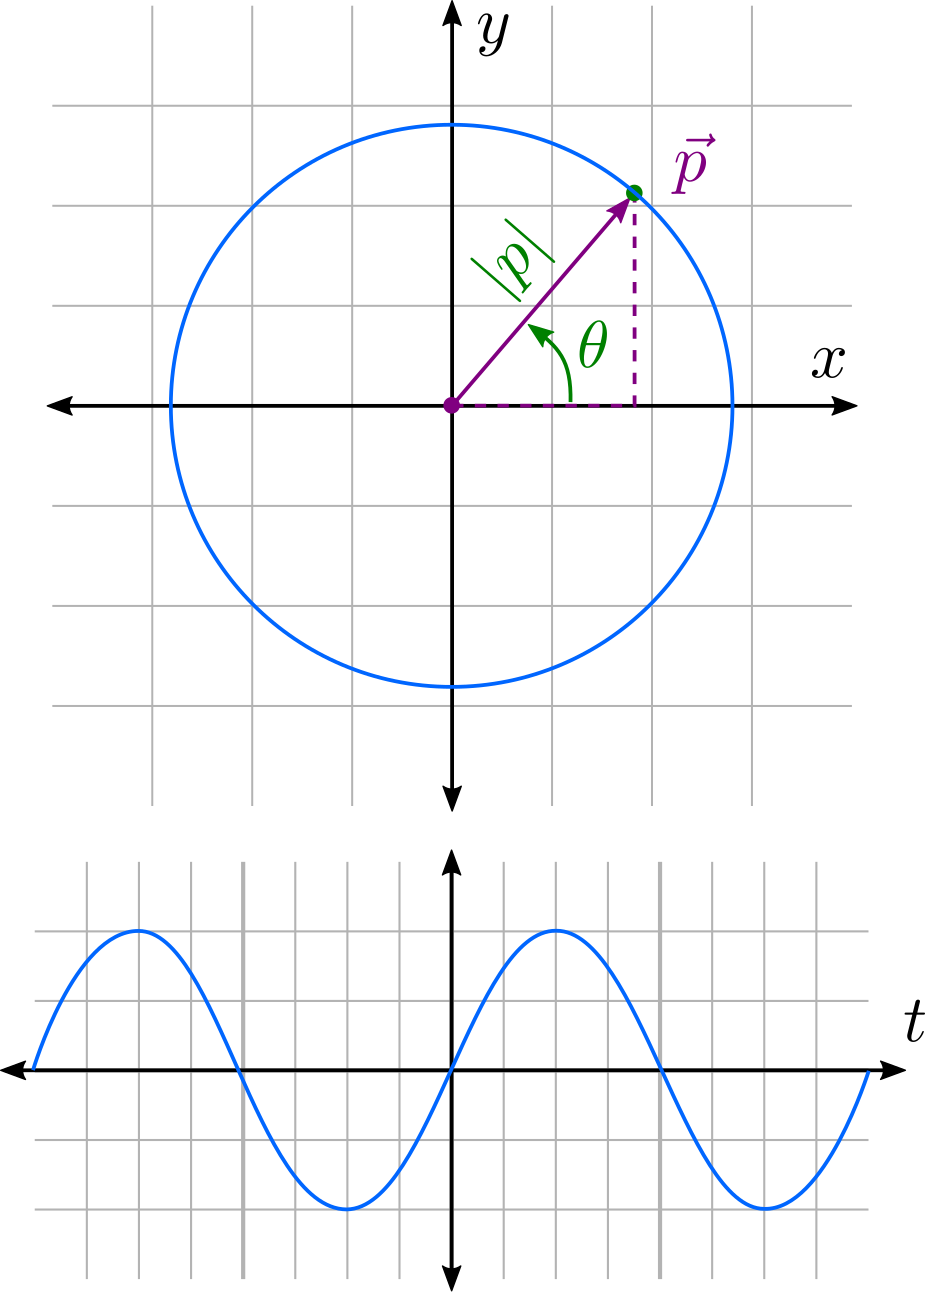
\includegraphics[scale=.16]{circular_frequency_fig2.png}

Frequency (\hspace{10mm}) and circular-frequency ($\hspace{10mm}$) are both commonly used.  \vspace{15mm}

You can easily convert from one to the other.
\end{multicols}

{\tiny Image: TH}
}

% Section 4
\section{Famous Example - Units Matter !!!}

\frame{
\frametitle{Famous Example - Units Matter !!!}

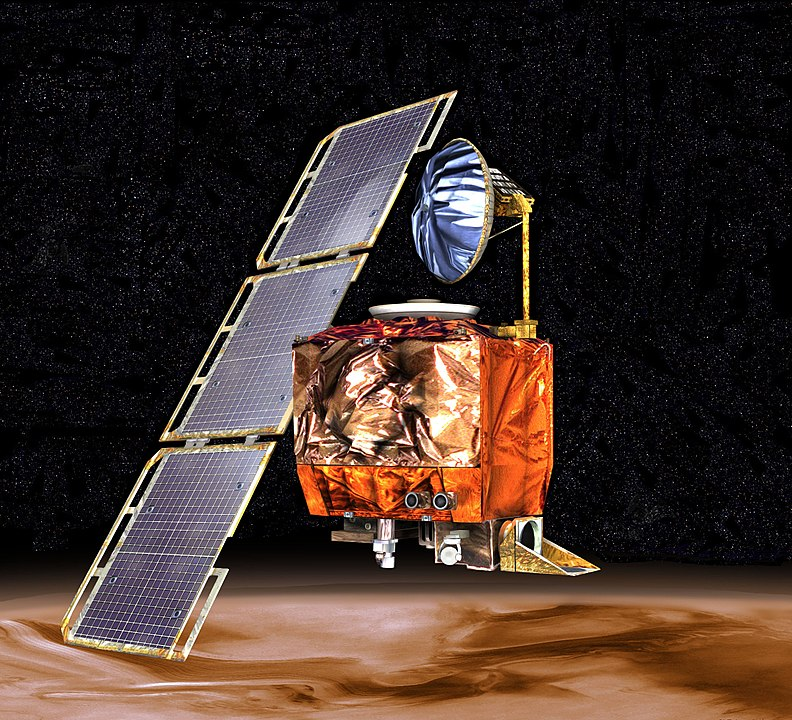
\includegraphics[scale=.1]{mars_orbiter.jpg}
The Mars Climate Orbiter (formerly the Mars Surveyor '98 Orbiter) was a 638-kilogram (1,407 lb)[1] robotic space probe launched by NASA on December 11, 1998 to study the Martian climate, Martian atmosphere, and surface changes and to act as the communications relay in the Mars Surveyor '98 program for Mars Polar Lander. {\tiny \href{https://en.wikipedia.org/wiki/Mars_Climate_Orbiter}{Full Story and Images: Wikipedia} }

}



\end{document}

	





